\chapter{Multijet background study}
\label{App:QCD_bkg_study}

The multijet suppression used in Section~\ref{subsec:ch7_multijet} is studied with simulated dijet and leptoquark events.
The motivation and discriminating variables are introduced there; this appendix presents the study selection, threshold scan and residual-background checks.

\section{Study selection and distributions}
\label{sec:app_qcd_selection}

The study selection is kept loose to retain enough simulated multijet events to examine the relevant distributions.
It requires the $\met$ trigger, exactly one hadronic $\tau$ candidate, no selected electron or muon, and at least one jet, as listed in Table~\ref{tab:app_qcd_preselection}.
The final SR thresholds on $\met$, $\pT^\tau$, $\mT$ and the visible invariant mass are not imposed at this stage.
No $b$-tag multiplicity is required.

\begin{table}[htbp]
    \centering
    \caption{Loose selection used to study the multijet suppression. This selection defines the denominator of the rejection fractions shown below.}
    \label{tab:app_qcd_preselection}
    \begin{tabular}{ll}
        \toprule
        Requirement & Selection \\
        \midrule
        Trigger & Lowest-threshold unprescaled $\met$ trigger \\
        Hadronic $\tau$ multiplicity & $N_\tau=1$ \\
        Electron and muon veto & $N_\ell=0$ \\
        Jet multiplicity & $N_j\geq1$ \\
        \bottomrule
    \end{tabular}
\end{table}

Figure~\ref{fig:app_qcd_correlations} shows the two-dimensional distributions after this selection.
The multijet sample is concentrated at small $\min\Delta\phi(j,\met)$ and relatively small $\met/\minDphiJetPt$.
The signal occupies a broader angular range and extends to larger momentum ratios.
Approximately $90\%$ of the multijet events have $\met/\minDphiJetPt<6$, compared with approximately $55\%$ of the signal in the study sample.
The ratio requirement alone would therefore reject a substantial fraction of the signal.
It is instead combined with the angular requirement so that either a large angle or a large ratio is sufficient to retain an event.

\begin{figure}[htbp]
    \centering
    \begin{subfigure}{0.49\linewidth}
        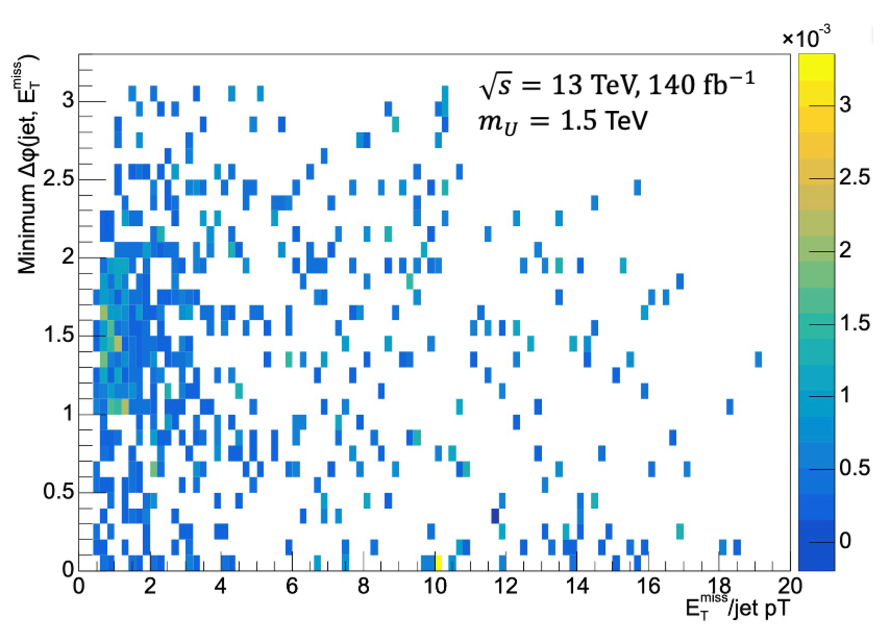
\includegraphics[width=\linewidth]{Figs/CH7/QCD/DPhi_signal.pdf}
        \caption{Signal.}
    \end{subfigure}\hfill
    \begin{subfigure}{0.49\linewidth}
        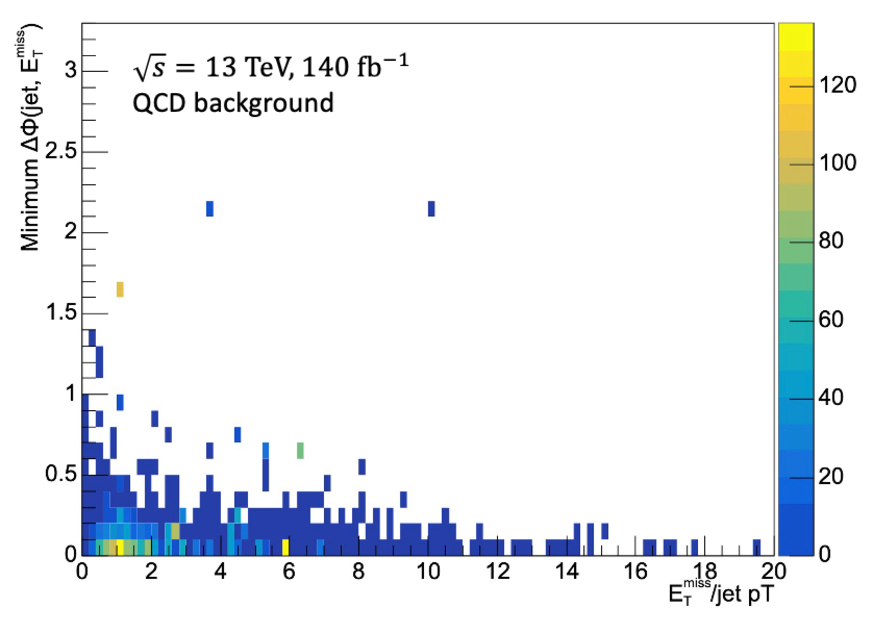
\includegraphics[width=\linewidth]{Figs/CH7/QCD/DPhi_multijets.pdf}
        \caption{Multijet background.}
    \end{subfigure}
    \caption[Variables used for multijet suppression]{Correlation between the minimum jet--$\mpt$ azimuthal separation and the ratio of $\met$ to the $\pT$ of the closest jet in azimuth, for (a) simulated signal with $\MU=1.5~\TeV$ and (b) simulated multijet background after the loose study selection. The concentration of multijet events at small values of both variables motivates a combined requirement.}
    \label{fig:app_qcd_correlations}
\end{figure}

\section{Threshold scan and signal retention}
\label{sec:app_qcd_scan}

The angular threshold is scanned while the momentum-ratio threshold is fixed at six.
For an angular threshold $X$, the rejected fraction is defined as
\begin{equation}
    \text{Rejection ratio}=\frac{N\!\left(\min\Delta\phi(j,\met)<X\ \text{and}\ \met/\minDphiJetPt<6\right)}{N(\text{all events after preselection})}.
    \label{eq:app_qcd_rejection}
\end{equation}
The numerator requires both small angular separation and a small momentum ratio.
Its complement is the accepted region, defined by the logical OR in Eq.~\ref{eq:ch7_qcd_cut}.
The rejected fraction is evaluated separately for signal and multijet events, using each sample's yield after the loose selection as its denominator.

Figure~\ref{fig:app_qcd_rejection_scan} shows the resulting rejection fractions.
At $X=0.4$, approximately $86\%$ of the multijet events are rejected, while the signal loss is $3.6\%$.
The corresponding signal efficiency for the cleaning cut is therefore $1-0.036=96.4\%$.
Increasing the angular threshold rejects more multijet events but also removes more signal.
The selected threshold provides substantial multijet rejection with a small signal loss in the studied sample.

\begin{figure}[htbp]
    \centering
    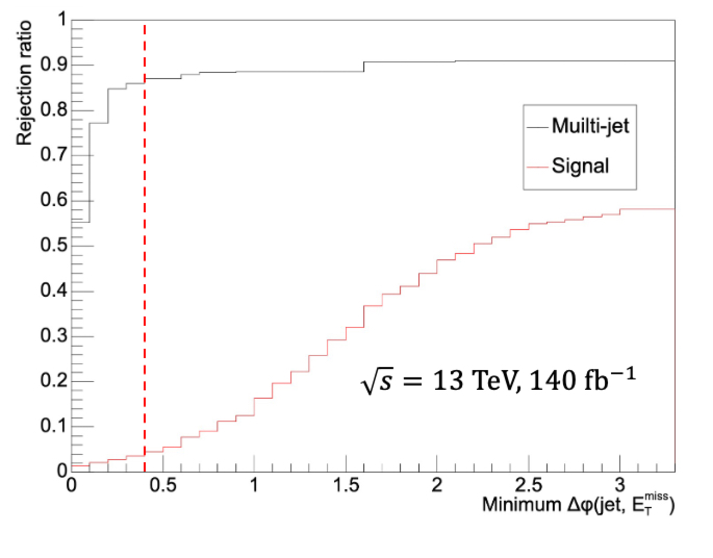
\includegraphics[width=0.70\linewidth]{Figs/CH7/QCD/rejection_scan.pdf}
    \caption[Scan of the multijet rejection threshold]{Rejected fractions of simulated signal and multijet events as a function of the minimum jet--$\mpt$ angular threshold $X$, with $\met/\minDphiJetPt<6$ also required in the rejected sample. The red and black curves show signal loss and multijet rejection, respectively. The vertical dotted line marks the adopted threshold $X=0.4$. The denominator is the loose selection in Table~\ref{tab:app_qcd_preselection}.}
    \label{fig:app_qcd_rejection_scan}
\end{figure}

\section{Residual multijet contribution}
\label{sec:app_qcd_residual}

The residual multijet contribution is examined after applying the cleaning cut and the full SR requirements.
No simulated multijet events survive those selections in the samples used for the study.
This supports neglecting the multijet contribution in the nominal SR prediction, but zero surviving simulated events does not establish an exactly zero physical rate or a quantitative upper bound without the effective sample size.

Jets misidentified as $\tau$ candidates can still occur in other background processes.
In particular, $Z\to\nu\nu$ production with jets contains genuine missing momentum and can pass the multijet cleaning even when the selected $\tau$ candidate is a jet.
This contribution is included in the simulated $Z$+jets background.
A supplementary selection requiring Medium $\tau$ identification while failing Tight also gives a negligible multijet contribution in the simulated study, supporting the effectiveness of the cleaning beyond the nominal Tight selection.
